\chapter{評価実験}
本章では，段階的に自己開示を促すことによる受容性の変化を検証するため，評価実験を行う．実験に用いる自己開示を促す楽曲推薦システムの設計・実装について述べ，実際に楽曲推薦システムを使用し，どのように評価を行うかについて述べる．

% 本章では，カラオケにおける自己開示のモデルを3軸で整理する．そして，この3軸に基づいた自己開示レベルの定義と分類方法について述べる．最後に，これらのモデルを実装した実験支援システムの詳細について説明する．

% -----------------------------------------------------------------------------------------
\section{実験設計}

本節では，実験目的，実験条件，実験手順について述べる．

\subsection{実験目的}
本実験は，段階的な自己開示支援が受容性の向上に与える効果を検証することを目的とする．提案手法が自己開示の深化と受容性の向上に寄与するかを明らかにするため，システムによる段階的支援の有無による比較実験を実施する．


\subsection{実験条件}

\subsubsection{実験環境}

実験はカラオケ空間をもした閉鎖的な空間で実施した．対面でのカジュアルな会話を促進するため，2つの座椅子を適度な距離を保って対面に配置し，Bluetoothスピーカーを通じて音楽を再生する．カラオケ店舗の雰囲気を模倣するため，YouTube\cite{youtube}で配信されているDAMチャンネル\cite{damchannel}の動画コンテンツを小音量で再生し，完全な無音空間を避けるようにした．また，実験室の壁面にプロジェクターでDAMチャンネルの映像を投影し，視覚的な要素も考慮した．照明は会話に支障をきたさない程度の明るさに調整することで，リラックスした雰囲気の実現を図った．

\begin{figure}[H]
    \centering
    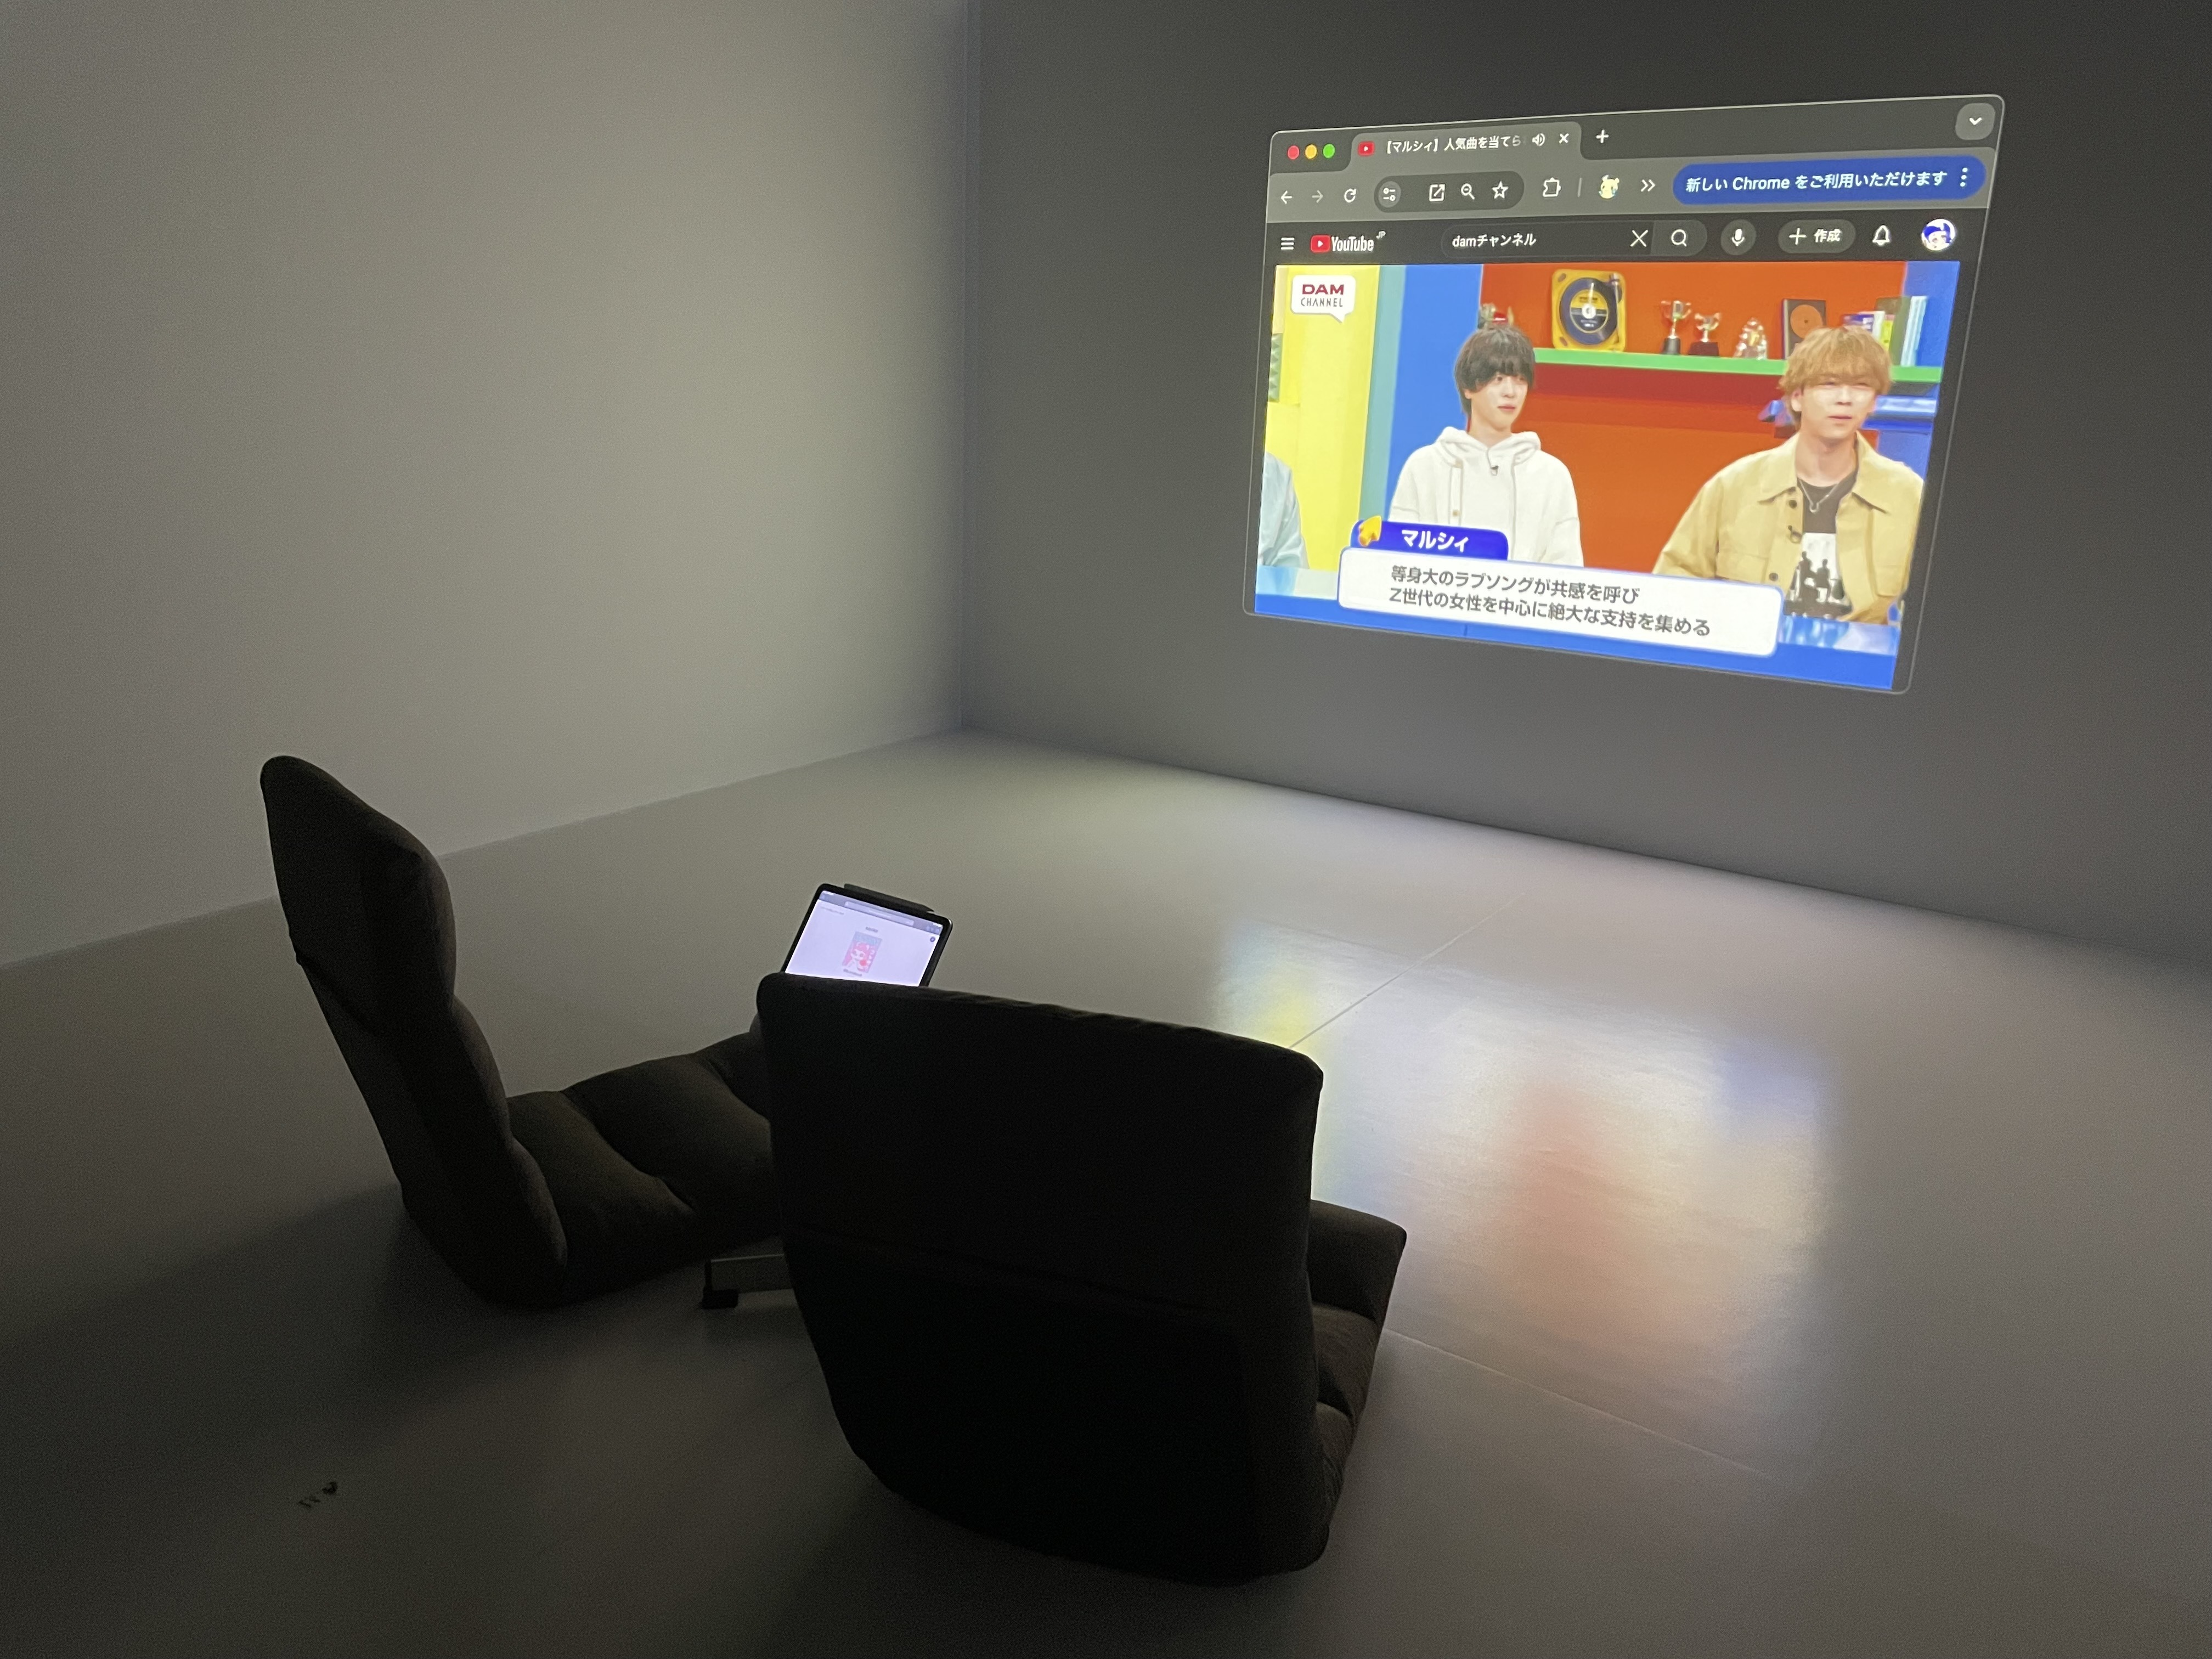
\includegraphics[width=0.75\linewidth]{image/実験環境.jpg}
    \caption{音楽共有セッションに用いる環境}
    \label{pic:実験環境}
\end{figure}


\subsubsection{実験参加者}
被験者は，年齢差がない学生・社会人の20名（18-24歳の男性8名，女性12名）を対象とし，10ペアで実験を行った．2群比較実験であるため，男女の比率が公平になるよう無作為に2群に割り当てた．

関係性は友人関係とした．友人関係とは，日常的な会話や活動を共にする程度でかつ，同じ空間で過ごしていても心理的負担を感じない関係性であり，自分の内面に関する深刻な悩み事を相談するほどの親密さには至っていない程度を対象とした．これは，初対面である場合は自己開示が重く感じられ，逆に親友レベルの関係性である場合はすでに深い自己開示を行えているため，友人という関係が最も適切であるとされている．


\subsection{実験手順}\label{実験手順}

音楽における自己開示の段階をレベル分けするため，選曲理由や楽曲にまつわる思い出の開示レベルを定義する．その後，このレベルに基づいて段階的に自己開示を促すシステムを実装する．

実験は事前準備と本実験の2段階で構成される．
事前準備では，被験者に50曲程度の「お気に入りの曲」プレイリストを作成してもらい，各楽曲に対する思い入れの強さを評価する．

本実験の音楽共有セッションでは，システムによる段階的な楽曲推薦を行う群（推薦あり群）と，支援を行わない群（推薦なし群）の2群で比較を行う．セッションは全8フェーズで構成され，各フェーズでは楽曲選択（推薦あり群はシステムが提示する候補から，推薦なし群は自身の作成したプレイリストの全楽曲から選択），楽曲再生，対話という流れで進行する．各フェーズ終了後，被験者は自己開示の度合いや楽曲体験の受容性に関する評価を行う．これらのデータを解析することで，段階的な自己開示が，相手の自己開示に対する受容性を向上させるかを検証する．

次節では，本実験で使用するシステムの設計・実装について詳しく説明する．
\section{自己開示を促す楽曲推薦システム}
本節では，システムの基本設計について述べる．

\begin{comment}
\subsection{要件}
選曲を通じた自己開示を促すには，システムに以下のような要件が必要である．

\subsection*{要件1. 個人の楽曲に対する自己開示レベルの定量化}
システムが自己開示を促進するうえでは，定量化する必要がある．

\subsection*{要件2. 段階的な自己開示の制御}
要件1で定量化した自己開示レベルについて，レベルの低い楽曲から高い楽曲へと段階的に開示を促す必要がある．

\subsection*{要件3. ユーザーの選曲過程や，受容度の変化を記録する}
要件2の段階的にシステムが提示した曲と，ユーザーの選択した曲の変化，すなわち要件1の自己開示レベルの変化を時系列的に記録できるシステムである必要がある．

\vskip\baselineskip

これらの要件を～．
\end{comment}

\subsection{3軸の分類基準}

本項では，\ref{3軸}項で整理した自己開示の3軸についての取得方法，定量化方法を検討する．「思い入れ」と「歌うことの自信」は，個人の主観であり，客観的指標として取得することが不可能である．そのため，主観指標として曲に対して表\ref{tab:evaluation_criteria}に示すように4段階で被験者に評価をさせることとした．

\begin{table}[htbp]
\centering
\caption{楽曲の評価基準}
\label{tab:evaluation_criteria}
\begin{tabular}{|c|c|c|}
\hline
評価値 & 思い入れ & 歌うことの自信 \\
\hline
1 & ほとんど思い入れがない & ほとんど自信がない \\
2 & あまり思い入れがない & あまり自信がない \\
3 & やや思い入れがある & やや自信がある \\
4 & とても強い思い入れがある & とても自信がある \\
\hline
\end{tabular}
\end{table}

楽曲の人気度については，個々人間で知っている/知らない曲を完全に網羅することは難しく，人により曲の認知度は違って感じられるため，主観指標を使うことは難しい．そのため，Spotify Web API\cite{SpotifyWebAPI}から取得できるpopularityという客観的な数値（0-100）を使用する．これら3つの指標に基づき，各楽曲の自己開示レベルを定量的に評価する．

次項では，各軸の数値から自己開示レベルを決定する方法について述べる．


\subsection{自己開示レベルの区分}

\ref{3軸}項での3軸に基づき，カラオケにおける自己開示を4つのレベルに分類する．既存の研究ではこのような自己開示の段階を定義した手法は存在しない．そのため，今回は各軸の値を活かすため，2分法を用いて表\ref{tab:自己開示レベルの分類}のように分類を行うこととした．

思い入れと歌うことの自信は，表\ref{tab:evaluation_criteria}の4段階評価から，1-2の値を低い，3-4を高いとする．人気度については，Spotify APIから取得した1-100の値を，50を閾値として高低の2値に変換する．なお，思い入れが低く（1-2），歌唱への自信も低く（1-2），人気度も低い（50未満）楽曲については，開示者の感情表現も乏しく，被開示者からの受容も得られにくいことから適切に機能しないと判断し，分類から除外する．
% この分類では，思い入れを主軸とし，歌唱への自信と人気度を補助的な要素として扱う．

\begin{table}[H]
\centering
\caption{自己開示レベルの分類}
\begin{tabular}{|c|c|c|c|}
\hline
自己開示レベル & 思い入れ & 歌える自信 &  人気度  \\
\hline
1 & ない & ある & 高い \\
\hline
1 & ない & ない & 高い \\
\hline
2 & ない & ある & 低い \\
\hline
2 & ある & ある & 高い \\
\hline
3 & ある & ない & 高い \\
\hline
3 & ある & ある & 低い \\
\hline
4 & ある & ない & 低い \\
\hline
- & ない & ない & 低い \\
\hline
\end{tabular}
\label{tab:自己開示レベルの分類}
\end{table}


\subsection{実装}
提案したシステム設計に基づき，Webアプリケーションとして実装を行った．本項では，使用した開発環境，事前準備と本実験のデータフローについて説明する．

\vskip.5\baselineskip

システムの実装には，表\ref{tab:libraries}に示すライブラリとフレームワークを使用した．アプリケーションのベースとしてNode.js 20.17.0を採用し，フロントエンド・バックエンドの統合フレームワークとしてNext.js\cite{NextJS}を使用した．
データベースにはSupabase\cite{Supabase}を採用し，データベース管理を行った．また，楽曲情報の取得にはSpotify Web APIを利用し，next-authとiron-sessionを用いてAPI認証を実装した．
本アプリケーションは実験被験者が実際に使用することを想定し，安定した運用環境としてVercel\cite{Vercel}を使用した．


\begin{table}[H]
\caption{システム作成に使用したライブラリ・バージョン}
\label{tab:libraries}
\begin{center}
\begin{tabular}{|l|c||l|c|} \hline
\multicolumn{4}{|c|}{Node.js 20.17.0} \\ \hline
ライブラリ & バージョン & ライブラリ & バージョン \\ \hline
@mui/material & 6.3.1 & @supabase/supabase-js & 2.47.10 \\
axios & 1.7.9 & iron-session & 8.0.4 \\
next & 15.1.3 & next-auth & 4.24.11 \\
react & 19.0.0 & tailwindcss & 3.4.1 \\
typescript & 5.7.2 & & \\ \hline
\end{tabular}
\end{center}
\end{table}

\ref{実験手順}項の実験手順を満たすような事前準備のデータフローを図\ref{fig:事前準備のデータフロー}に，本実験の音楽共有セッションでのデータフローを図\ref{fig:音楽共有セッションのデータフロー}に示す．

\begin{figure}[H]
    \centering
    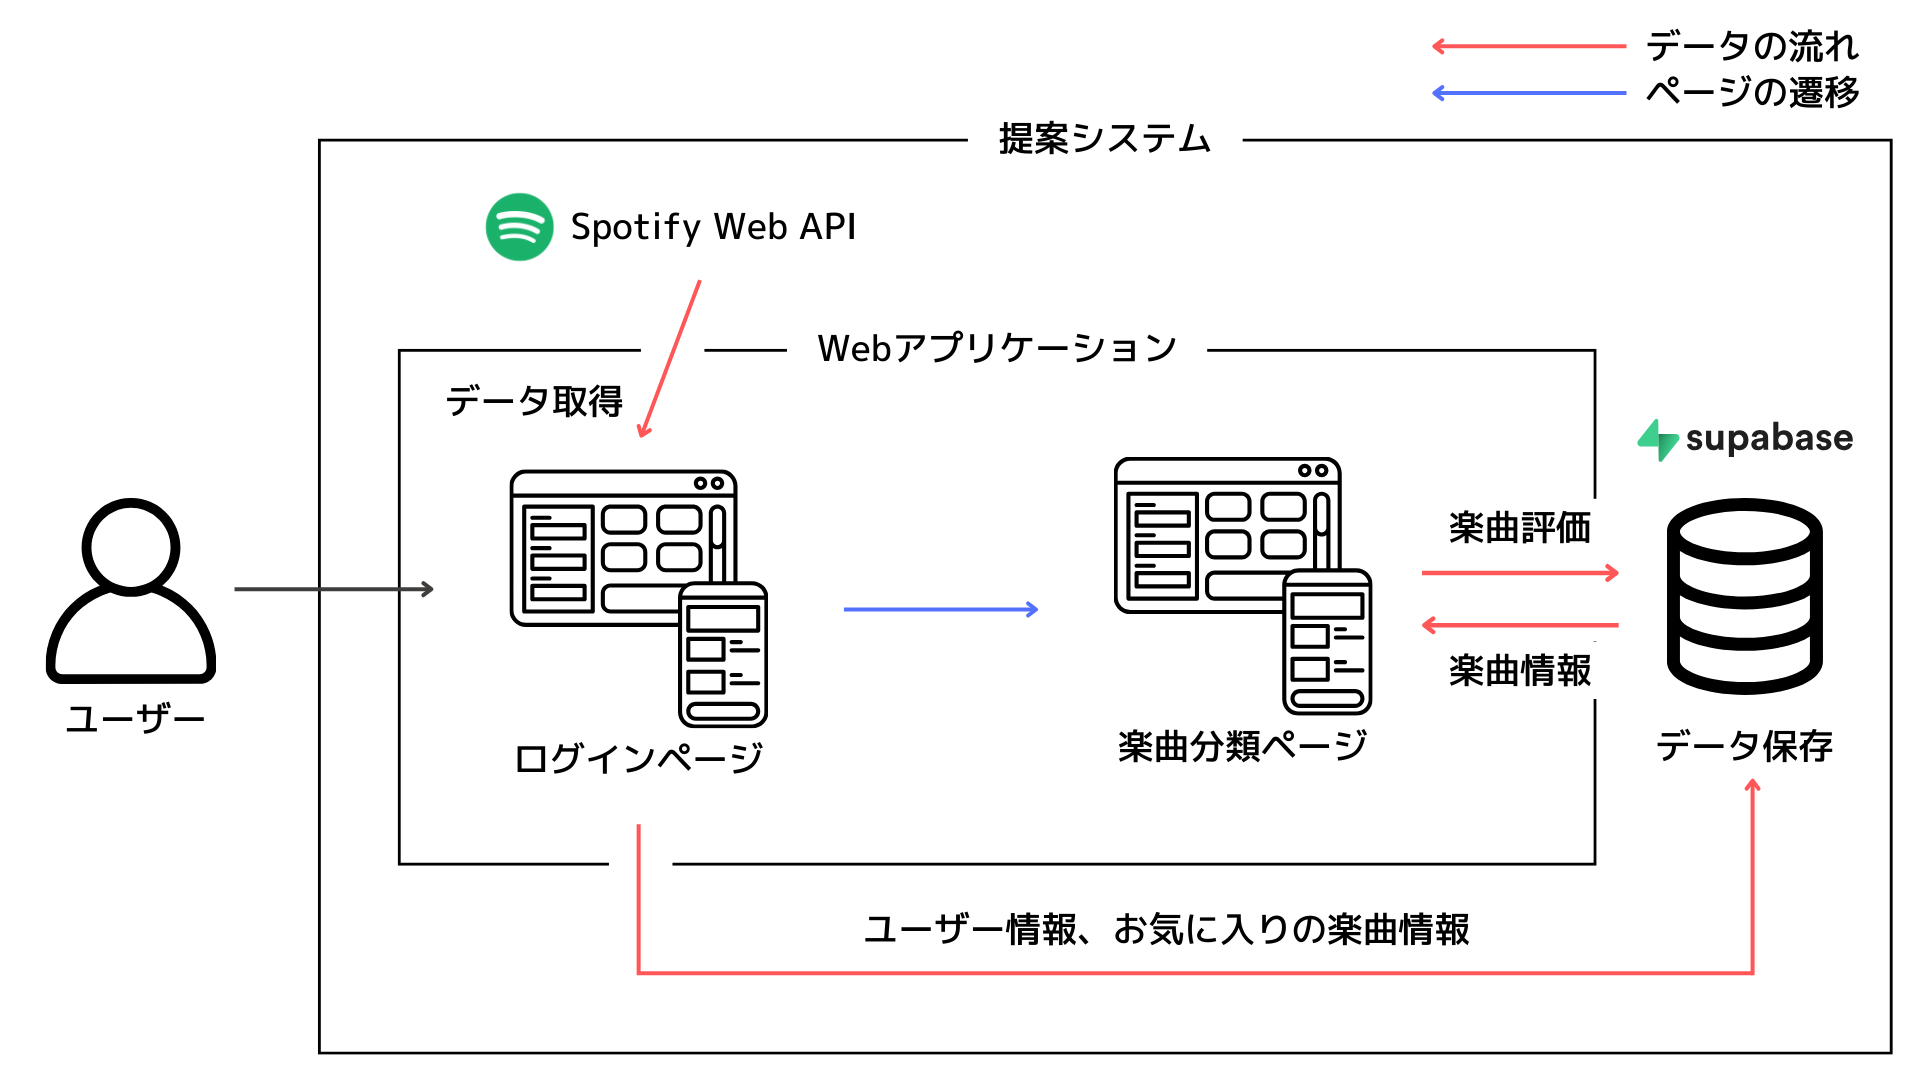
\includegraphics[width=1\linewidth]{image/data-flow-chart1.png}
    \caption{事前準備のデータフロー}
    \label{fig:事前準備のデータフロー}
\end{figure}

\begin{figure}[H]
    \centering
    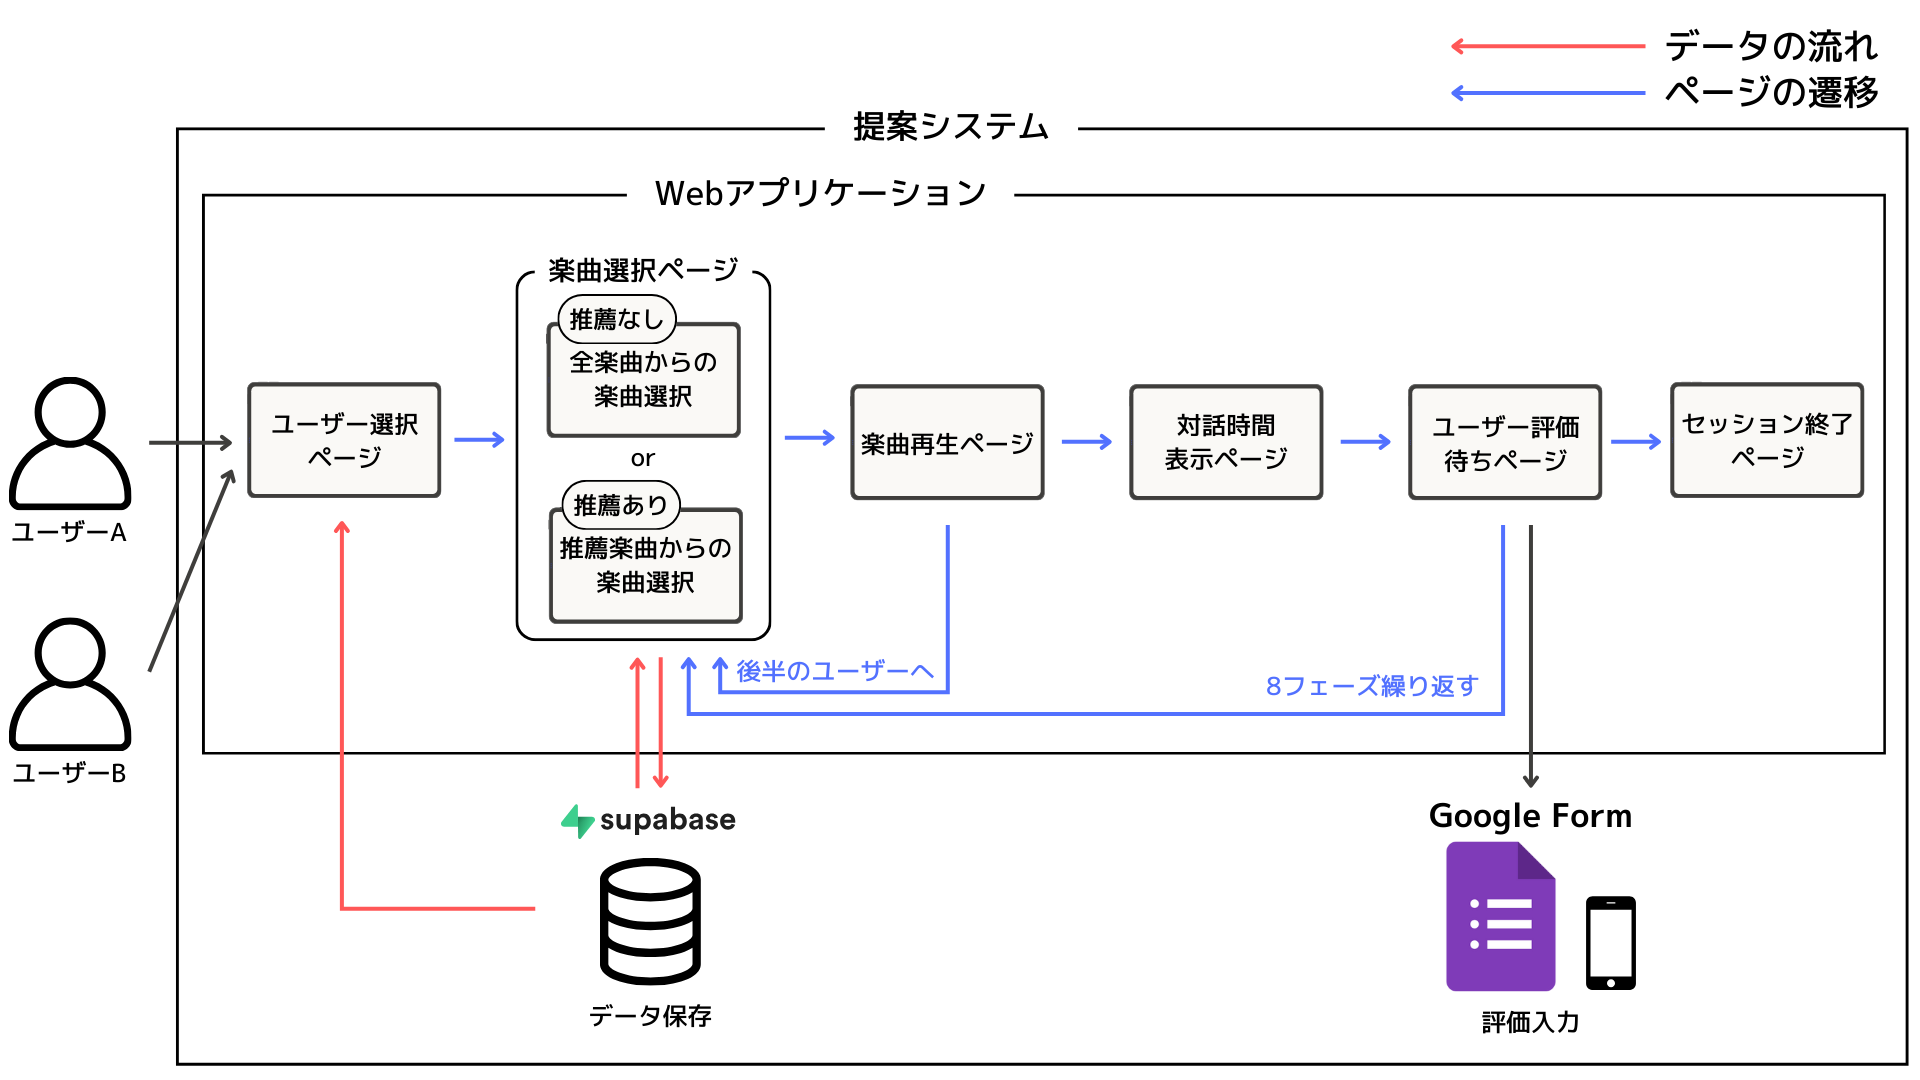
\includegraphics[width=1\linewidth]{image/data-flow-chart2.png}
    \caption{音楽共有セッションのデータフロー}
    \label{fig:音楽共有セッションのデータフロー}
\end{figure}

\section{実験方法}
実験は事前準備と本実験の2段階で構成される．
本実験では，システムによる段階的な楽曲推薦を行う群（推薦あり群）と，支援を行わない群（推薦なし群）の2群で比較を行う．

\subsection{事前準備}

事前準備では，被験者に実験用のSpotifyアカウントを作成してもらい，50曲程度の「お気に入りの曲」プレイリストを作成する．その後，Webアプリケーションを用いて，図\ref{fig:song_classification}に示した楽曲分類画面で，各楽曲に対する思い入れの強さと歌唱への自信を4段階で評価する．ユーザーの作業の負担を考慮し，楽曲分類の際には途中で保存ができる機能を実装した．

また，図\ref{fig:classified_songs}に分類済みの楽曲一覧を確認できる画面を示す．この画面では，分類が完了した楽曲の一覧を表示する．被験者は，自身が分類した楽曲を確認することができる．また，再度の分類もできるようにした．

\begin{figure}[H]
   \centering
   \begin{minipage}[b]{0.45\linewidth}
       \centering
       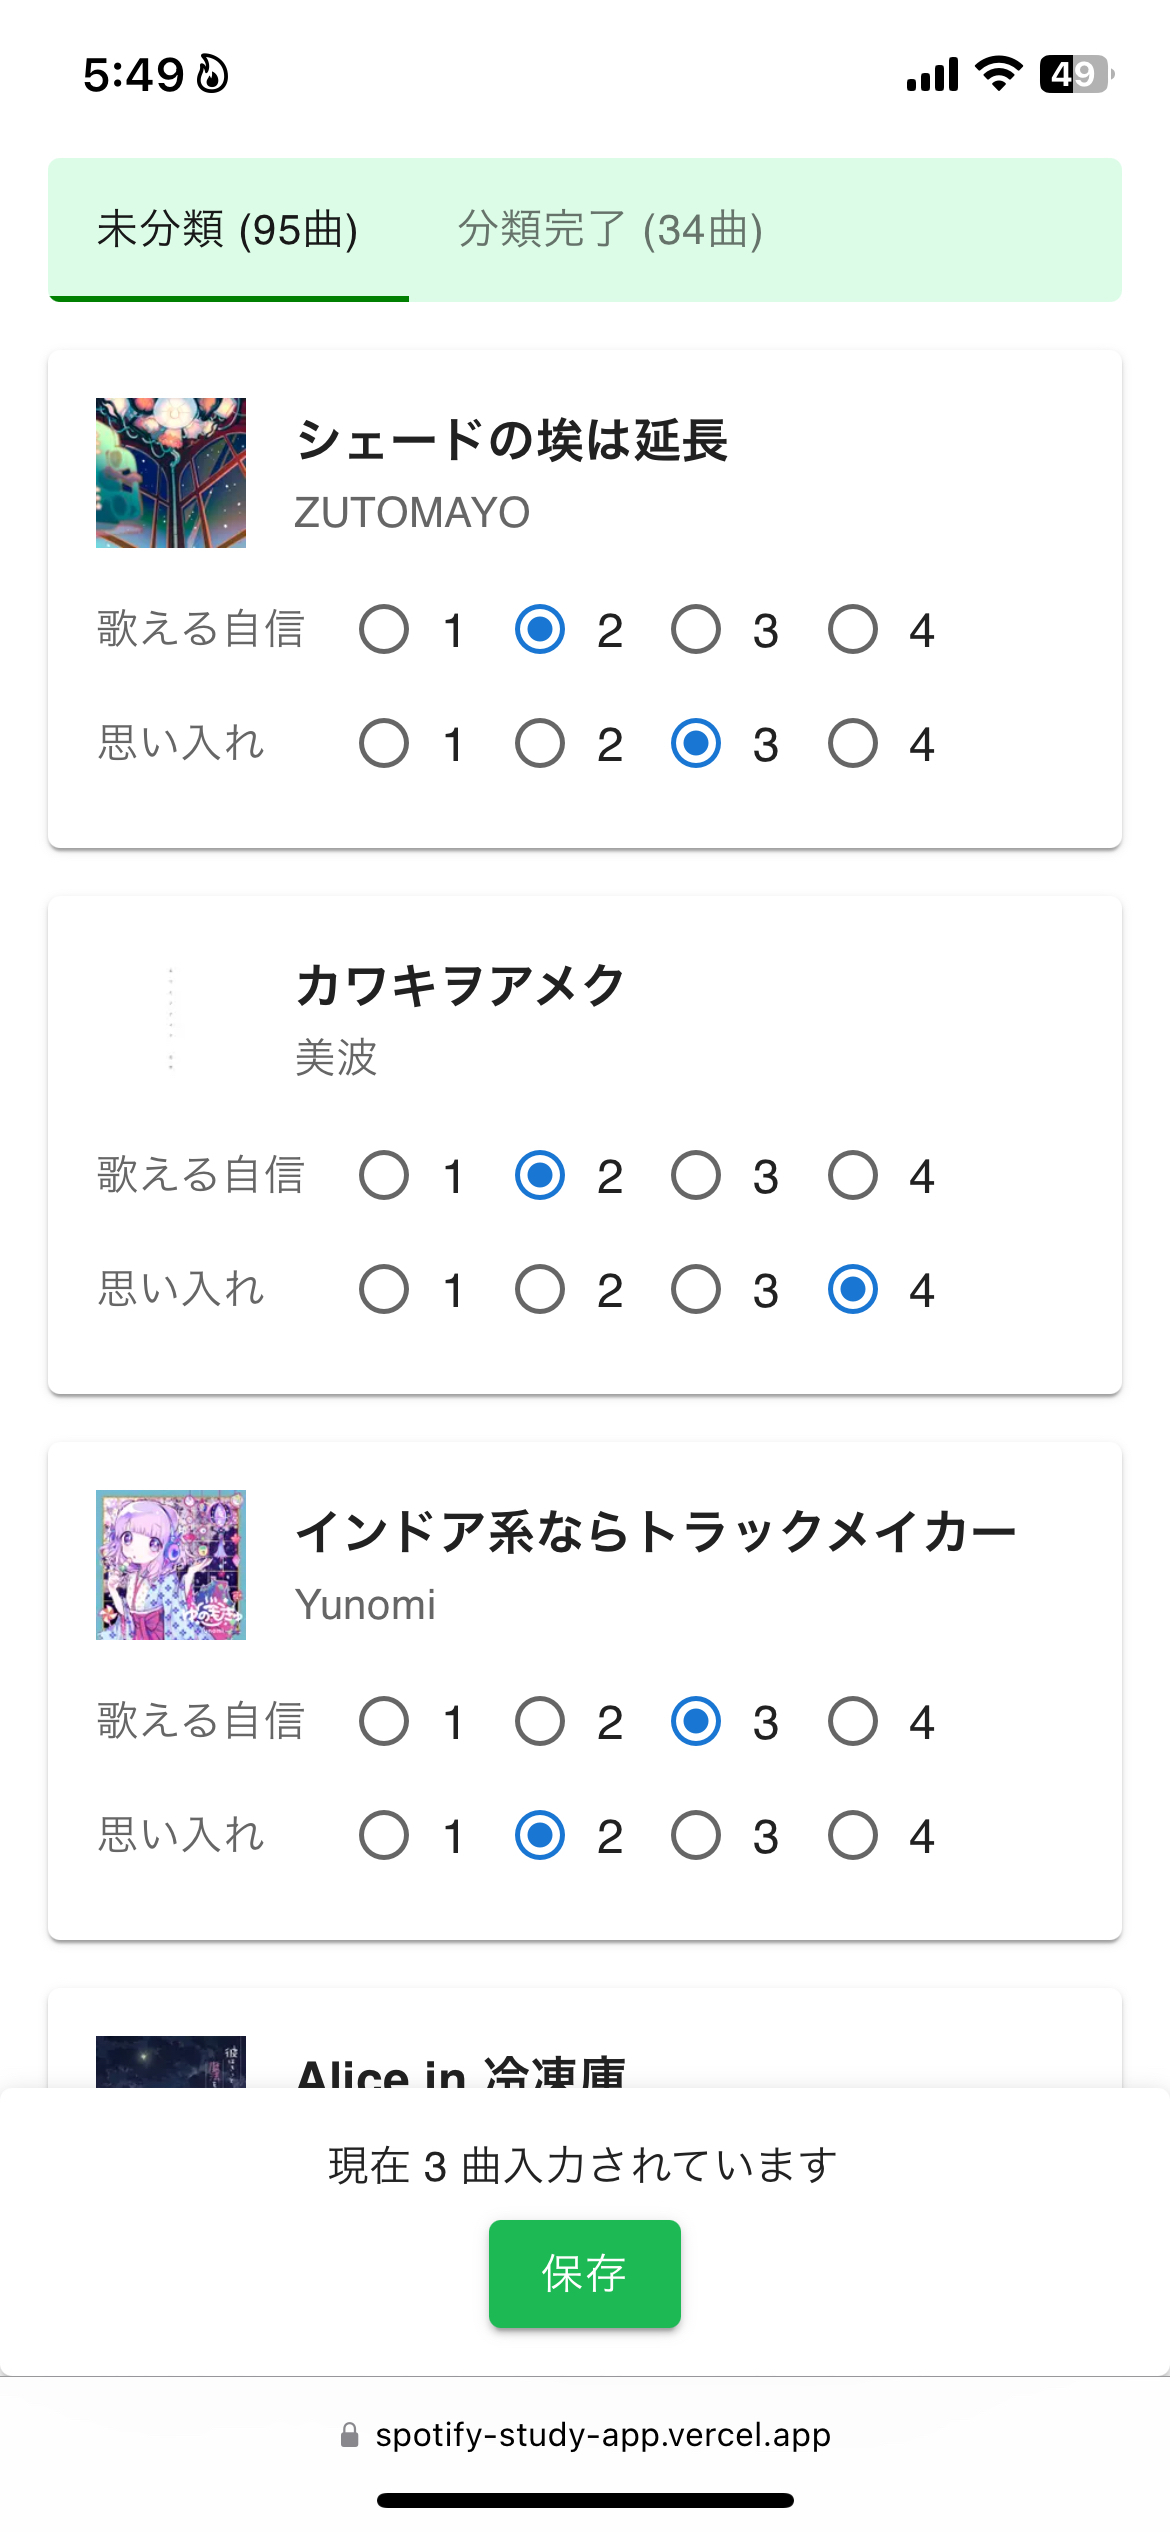
\includegraphics[width=0.9\linewidth]{image/ss_未分類.png}
       \caption{楽曲分類画面}
       \label{fig:song_classification}
   \end{minipage}
   \hfill
   \begin{minipage}[b]{0.45\linewidth}
       \centering
       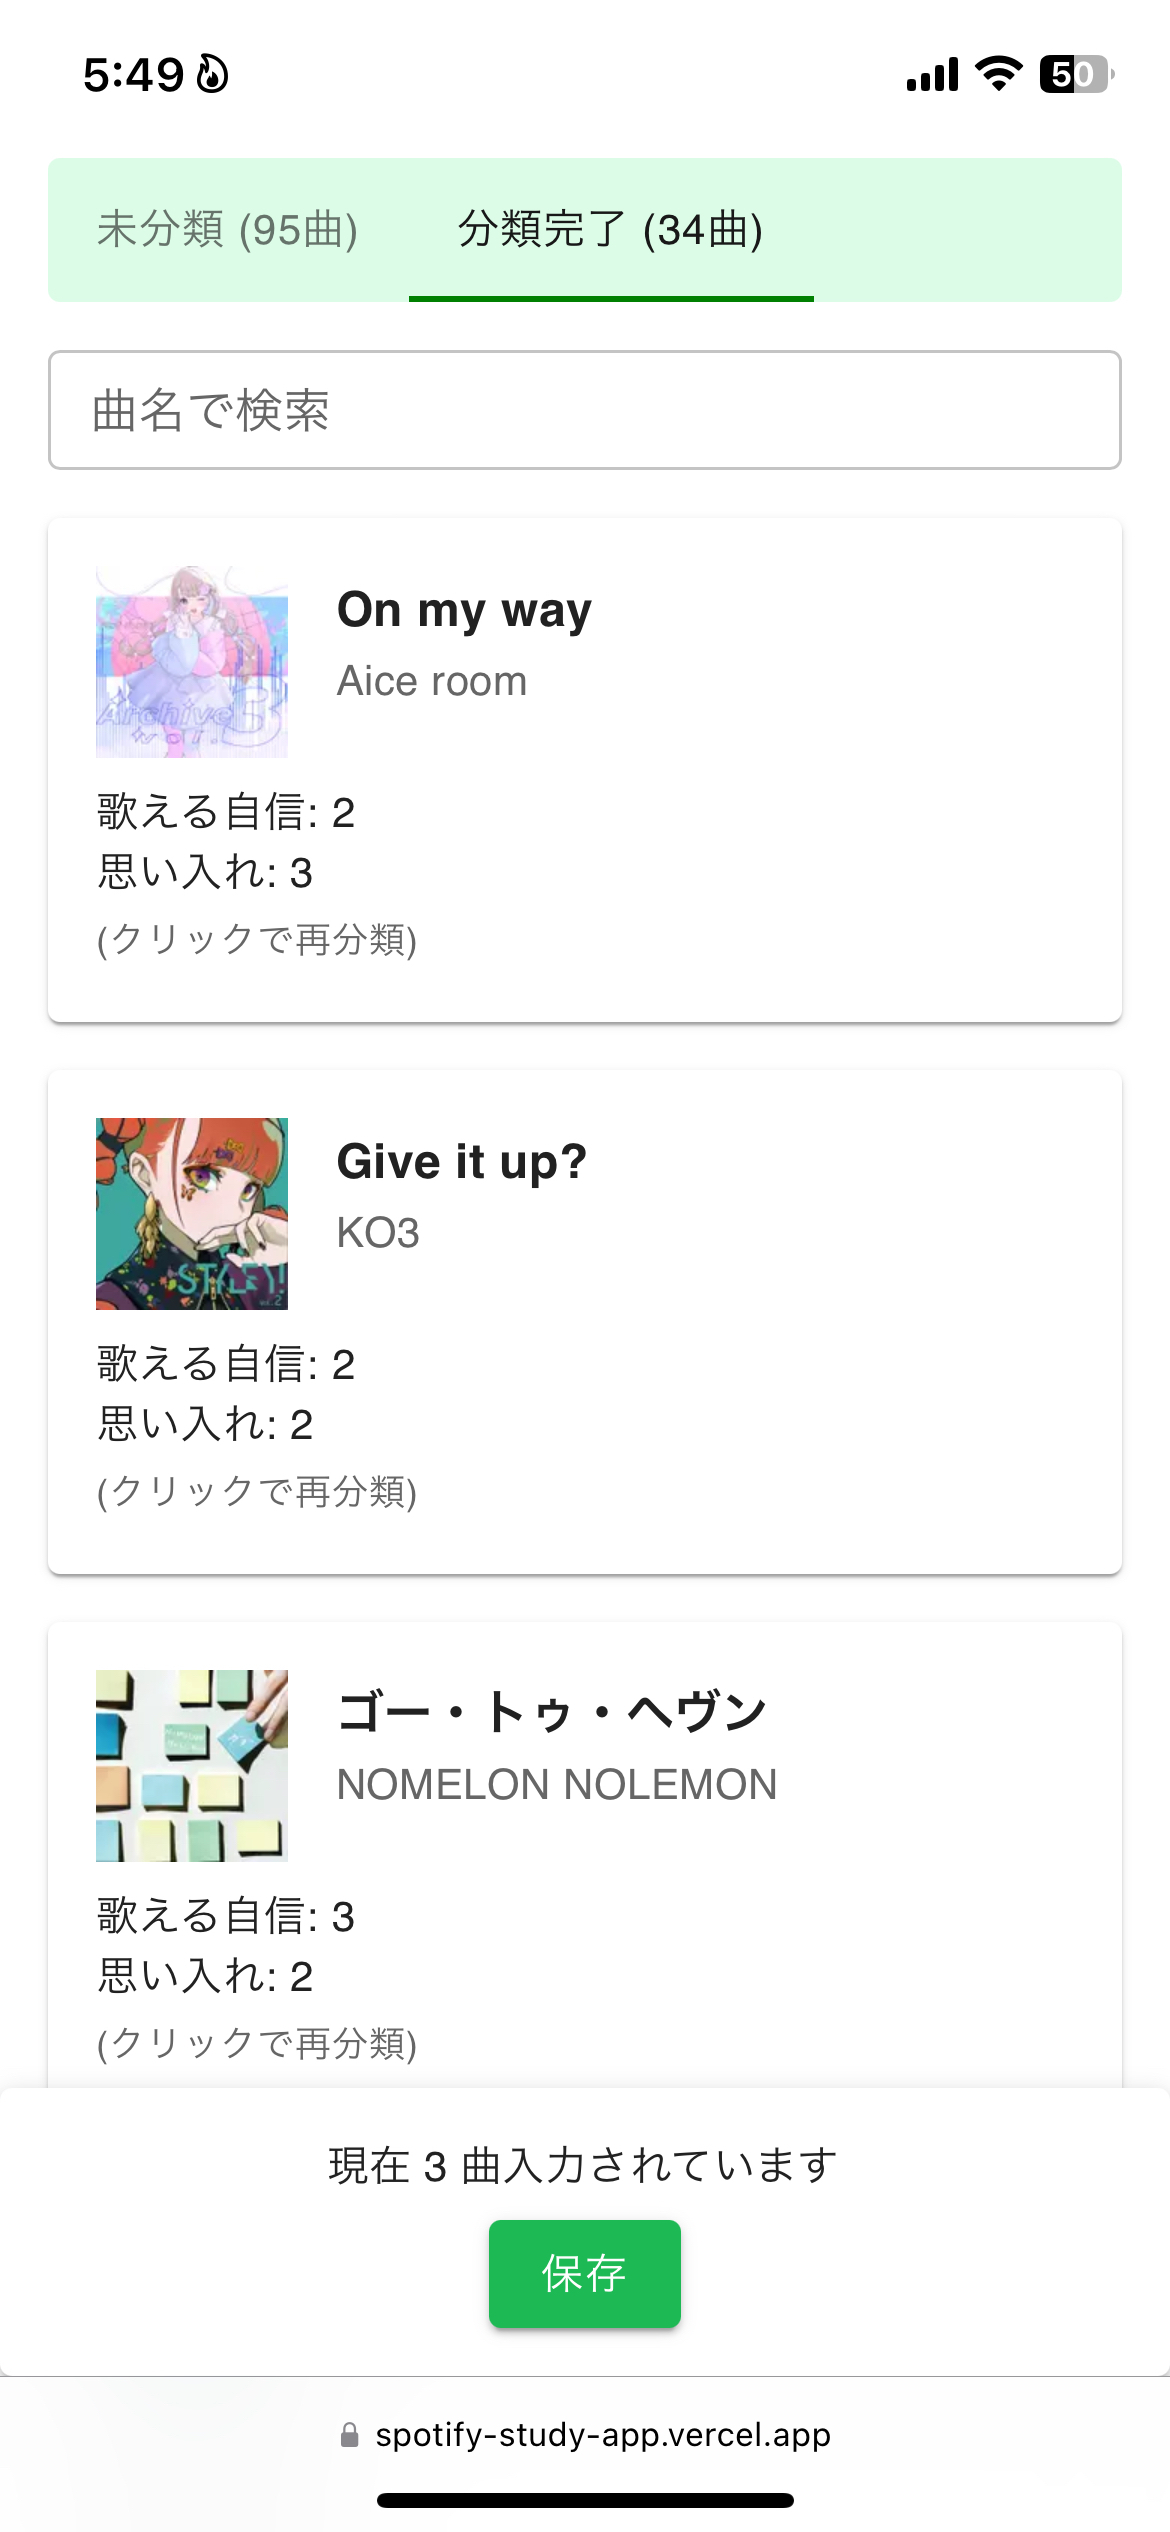
\includegraphics[width=0.9\linewidth]{image/ss_分類済み.png}
       \caption{分類済み楽曲一覧画面}
       \label{fig:classified_songs}
   \end{minipage}
\end{figure}


\subsection{本実験}

各被験者ペアを，本学の実験環境に案内し，互いに横並びになる形で座椅子に着席させる（図\ref{pic:実験環境}参照）．被験者に対して実験手順と注意点について説明し，音楽共有セッションを開始するよう指示をする．音楽共有セッションについては，以下の説明を行う．

\vskip.5\baselineskip

\textbf{推薦なし群:}
このセッションでは，あなたの音楽の好みについて相手と共有していただきます．
好きな曲をリストから選んで，選んだ曲を一緒に聴いたあと，その曲についてお話しください．曲にまつわる思い出や感想など，自由に会話を楽しんでください．

\vskip.5\baselineskip

\textbf{推薦あり群:}
このセッションでは，音楽を通じたコミュニケーションを体験していただきます．
システムが，あなたの音楽の興味や好みに基づいた曲の候補を提示します．
提示された候補の中から，共有したい曲を選んでください．
選んだ曲を一緒に聴いたあと，その曲についてお話しください．曲にまつわる思い出や感想など，自由に会話を楽しんでください．

\vskip.5\baselineskip

音楽共有セッションは全8フェーズで構成される．各フェーズは2ターン制を採用しており，以下の流れで進行する：

\begin{itemize}
    \item 第1ターン：被験者Aが開示者となり，被験者Bが被開示者となる
    \item 第2ターン：被験者Bが開示者となり，被験者Aが被開示者となる
\end{itemize}

つまり，1フェーズは「被験者A→被験者B」「被験者B→被験者A」という順序で2回の自己開示が行われる．

各ターンは，以下の3つのステップにより構成される．

\begin{enumerate}
    \item 楽曲選択フェーズ（30秒）
    \begin{itemize}
        \item 推薦なし群：事前に作成した個人のプレイリストから任意の1曲を選択する（図\ref{fig:free_selection}）
        \item 推薦あり群：システムが推薦する4曲の中から1曲を選択する（図\ref{fig:recommendation}）
    \end{itemize}
    
    \item 楽曲再生フェーズ（30秒）
    \begin{itemize}
        \item 選択楽曲を再生する．開示者が好きな場所から再生することができる
    \end{itemize}
    
    \item 対話フェーズ（60-90秒）
    \begin{itemize}
        \item 選曲理由や楽曲にまつわる思い出などを自由に共有し対話する
    \end{itemize}
    
\end{enumerate}

1フェーズが終わるごとに，GoogleForms\cite{googleforms}を利用して開示者と被開示者の双方が評価を行う．

\vskip.5\baselineskip

\begin{figure}[H]
    \centering
    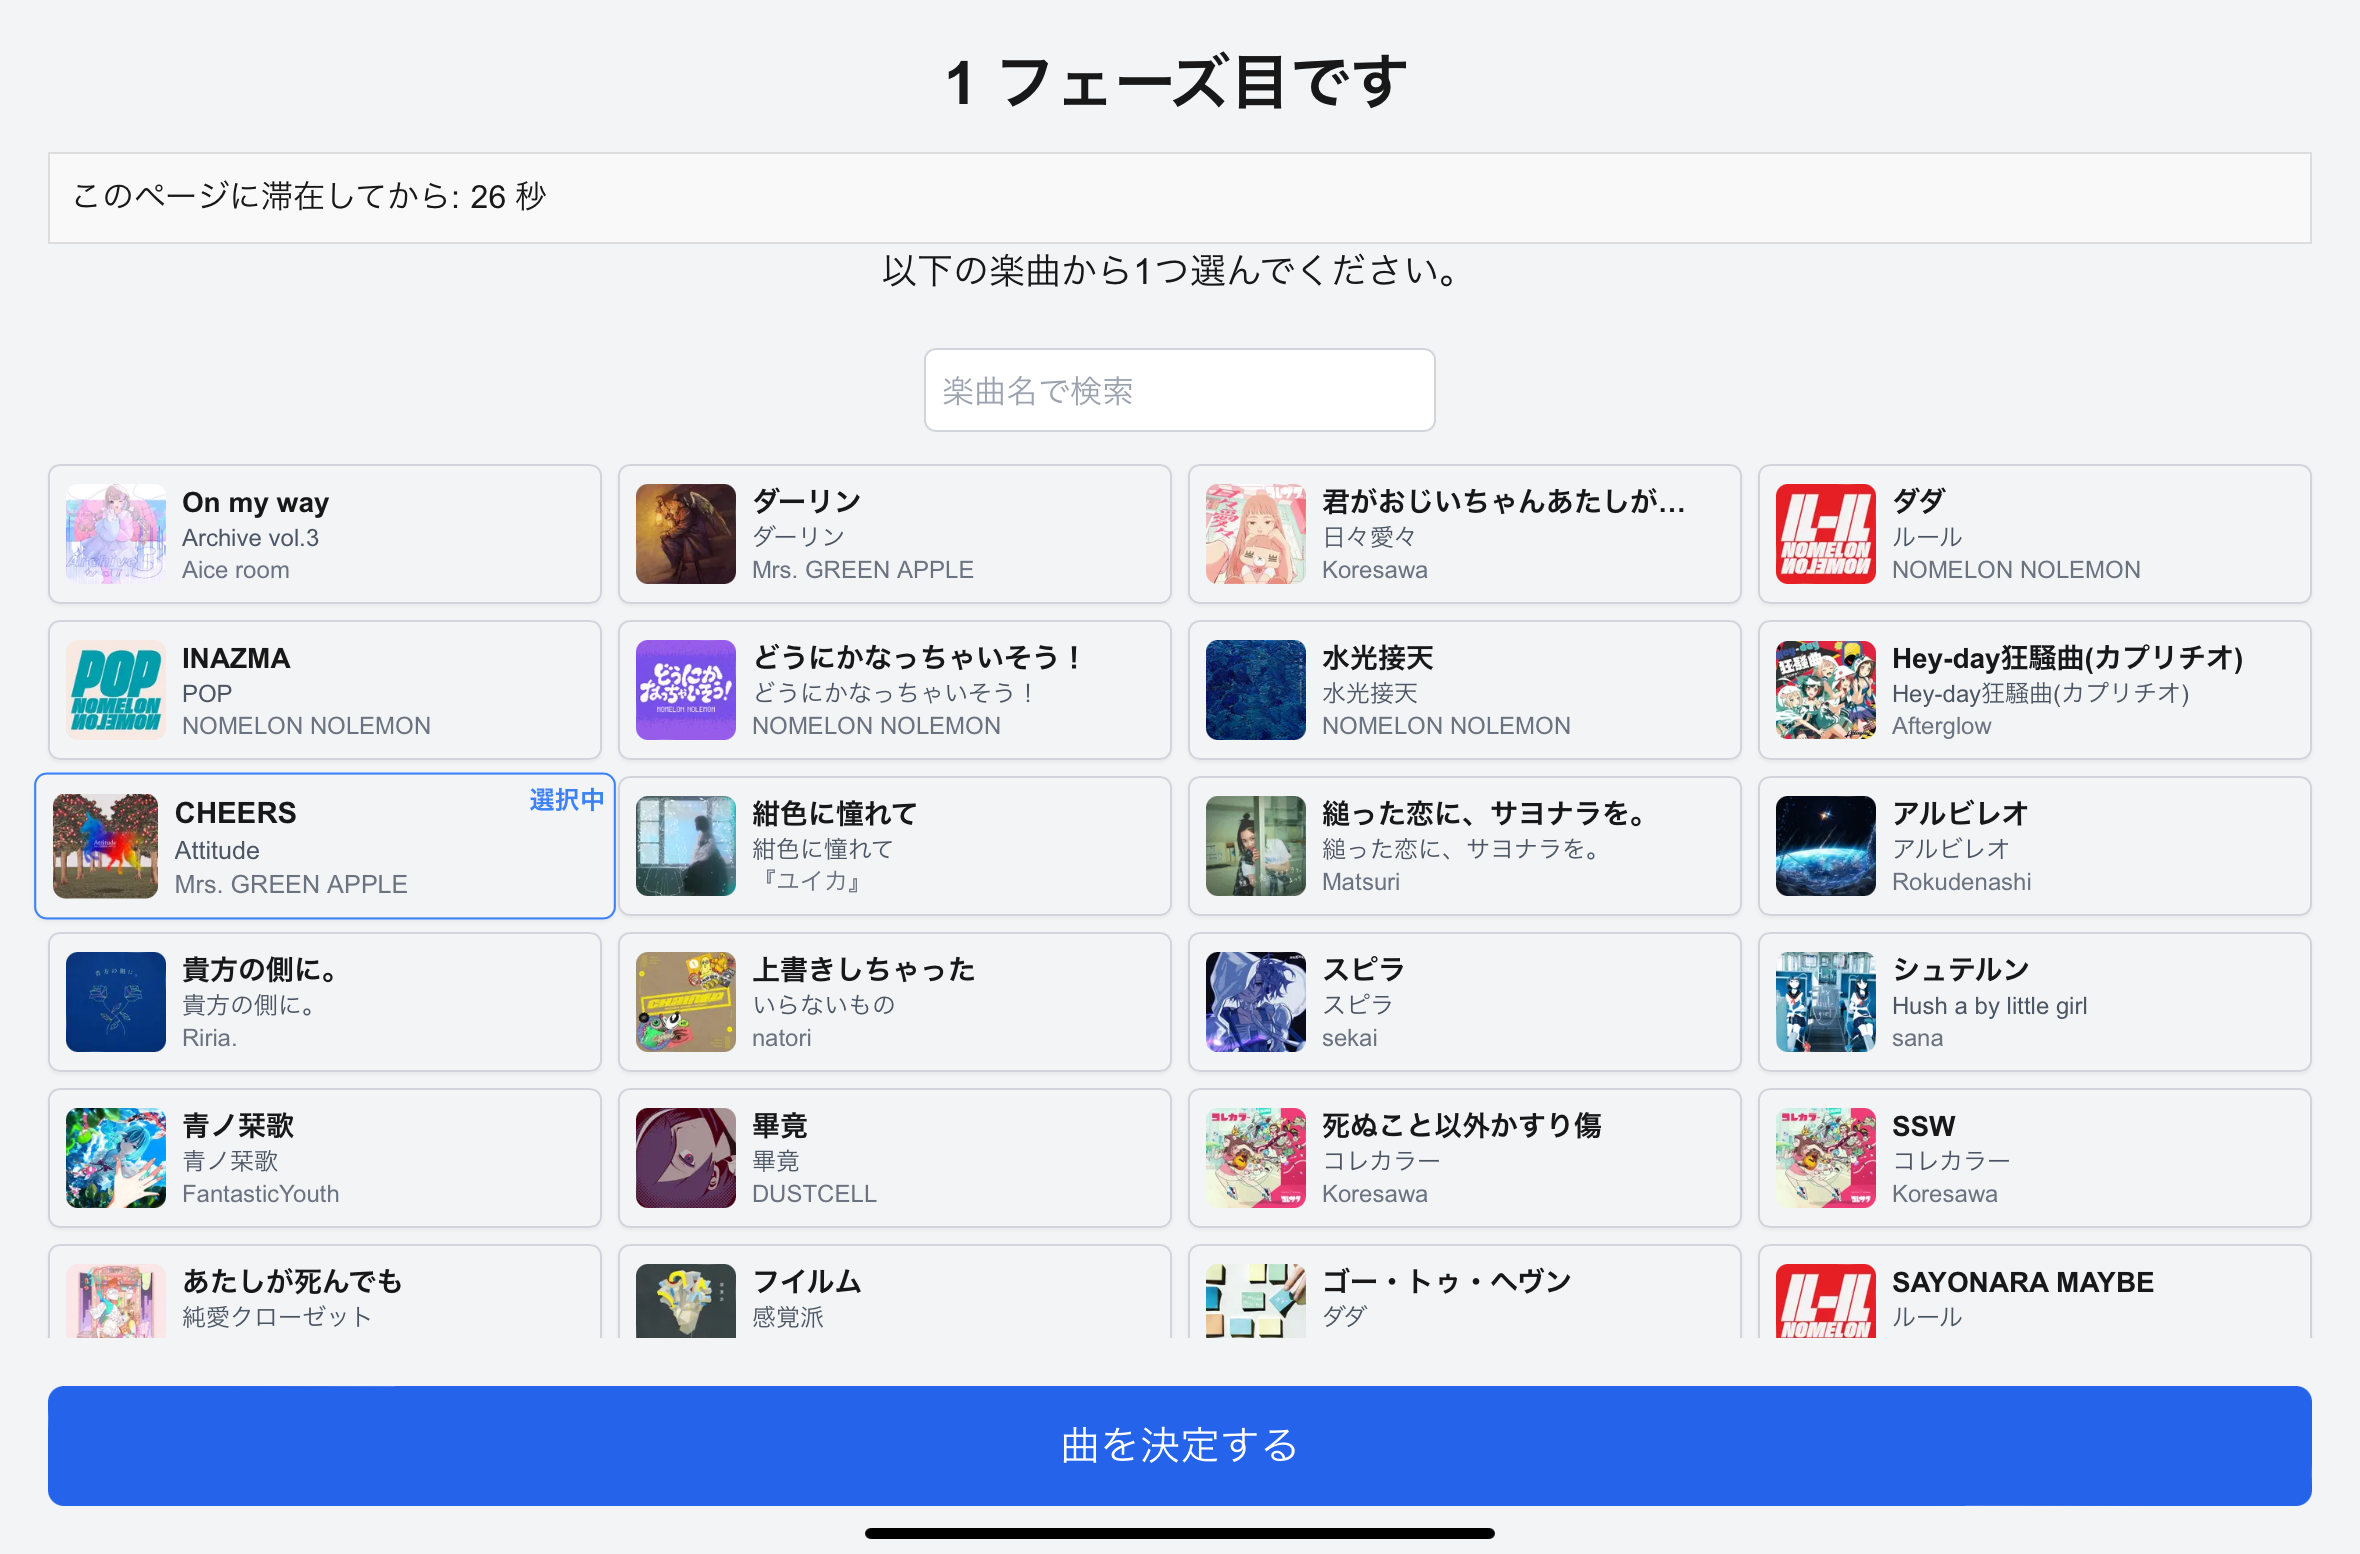
\includegraphics[width=0.9\linewidth]{image/ss_推薦なし_選曲.png}
    \caption{自由選択画面（推薦なし群）}
    \label{fig:free_selection}
\end{figure}

\begin{figure}[H]
    \centering
    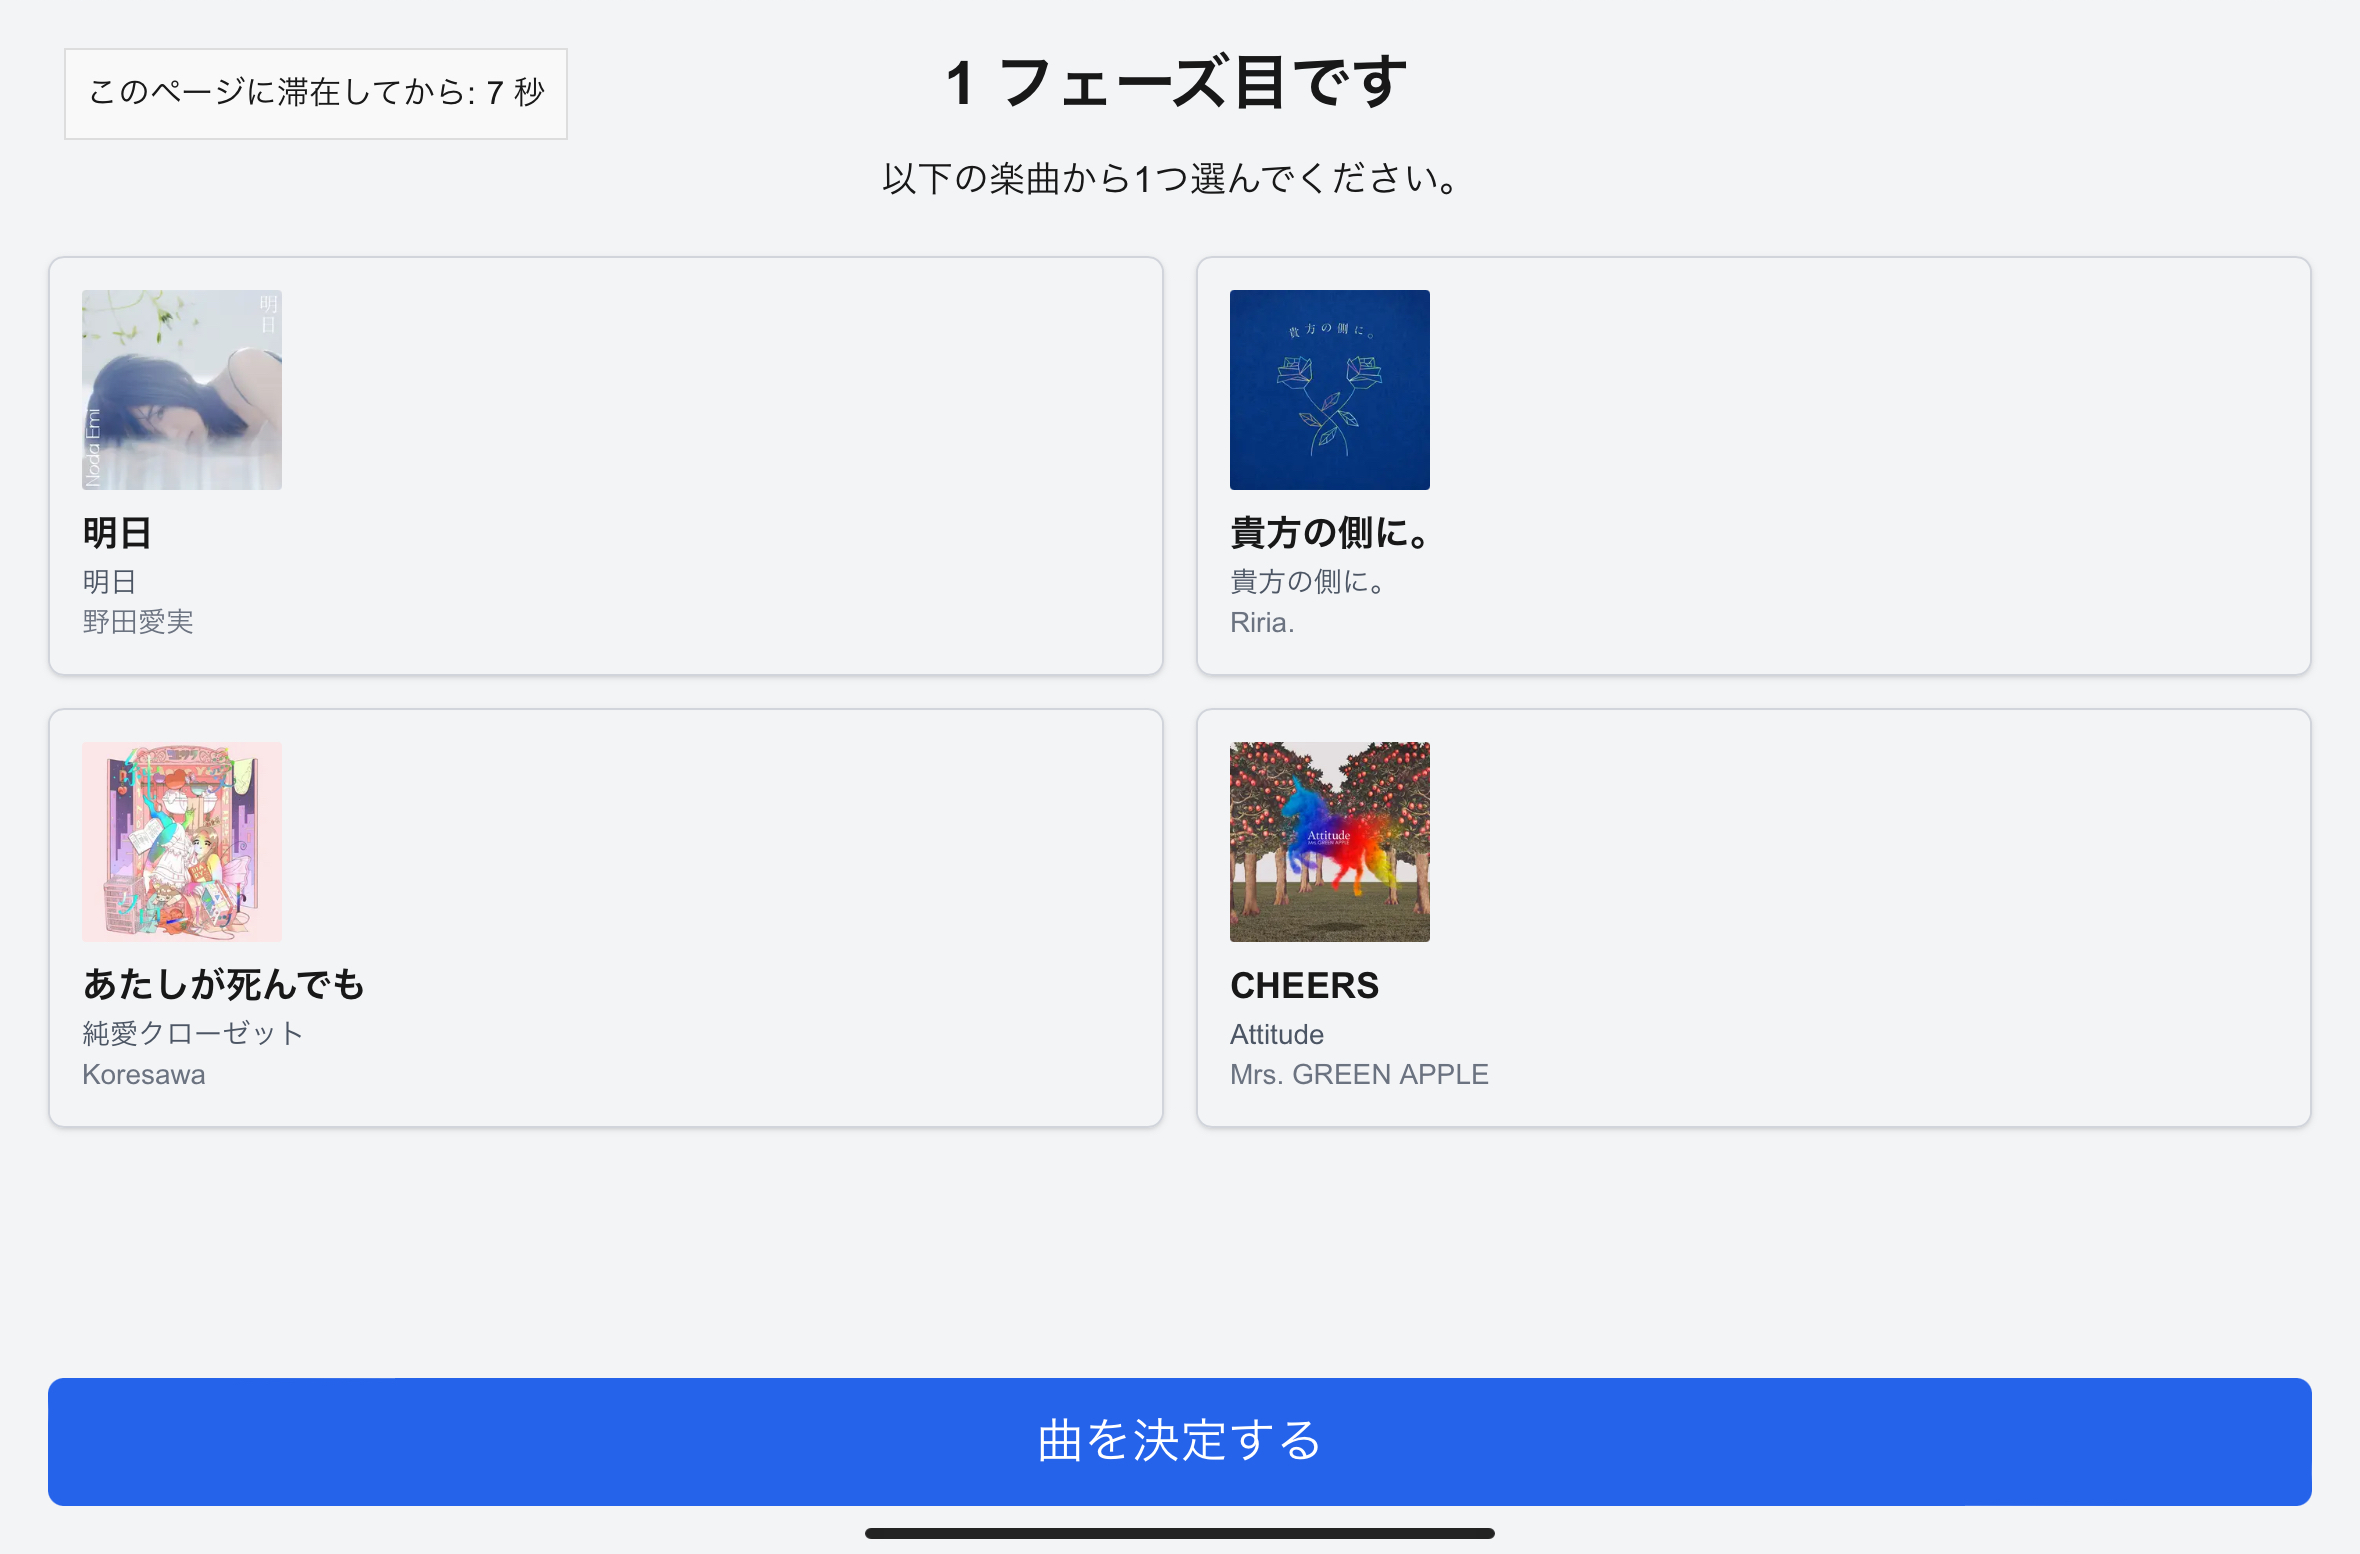
\includegraphics[width=0.9\linewidth]{image/ss_推薦あり_選曲.png}
    \caption{楽曲推薦画面（推薦あり群）}
    \label{fig:recommendation}
\end{figure}


% \subsection*{注意点}
% あとでくわしくかく

\section{評価方法}

\ref{研究課題と仮説}節で述べた仮説を検証するため，実験を実施するうえで以下の4つの指標について評価を実施する．

\vskip.5\baselineskip

\textbf{自己開示レベル:}自己開示のレベルの推移を明らかにするため，システムログより，各フェーズでの選曲履歴を取得する．
\vskip.5\baselineskip

\textbf{受容度:}仮説1, 2を検証するため，受容性の評価は，被開示者側と開示者側の両面から測定を行う．表\ref{実験中のアンケート項目}に，実験中のアンケート項目を示す．被開示者に対して，相手の自己開示をどの程度理解し，受け入れることができたかについて，表\ref{実験中のアンケート項目}のEQ1, EQ2を使用する．また，開示者側が知覚した相手からの受容についても取得することとして表\ref{実験中のアンケート項目}のEQ5, EQ6を使用する．これにより，段階的な自己開示が受容性に与える効果を，定量的に分析することができる．

また，実験終了後に相手の自己開示に対する印象や，理解が深まった点について表\ref{実験後のアンケート項目}のアンケートを行う．具体的には，相手に対する理解度，相手の音楽の好みに対する理解度，今後も相手と音楽を通じた会話をしたいと思うかを評価項目として設定する．
\vskip.5\baselineskip

\textbf{曲への興味:}仮説2を検証するため，被開示者に対し，選択された楽曲を知っていたかどうか（EQ3）と，相手の曲に興味を持てたかどうか（EQ4）という指標で相手の選曲に対しての評価を行う．これにより，音楽への興味度と受容性の関係性を分析する．
\vskip.5\baselineskip

\textbf{被験者の意見:}実験後のヒアリング項目を表\ref{実験後のヒアリング項目}に示す．選曲の意識，セッション全体の雰囲気，フェーズ前半と後半での違いなどについて，被験者からの主観的な評価を収集する．

\vskip\baselineskip

アンケートは，一部はい，いいえの2値や複数選択の回答があるが，明記していないものはすべて5段階評価（1:全くそう思わない ～ 5:とてもそう思う）を使用している．

\begin{table}[H]
  \caption{実験中のアンケート項目（EQ）}
  \label{実験中のアンケート項目}
  \centering
  \begin{tabular}{|l|p{0.85\textwidth}|}
    \hline
     & \textbf{質問内容} \\
    \hhline{|=|=|}
    EQ1 & 流した曲について楽しく話ができた \\
    \hline
    EQ2 & 相手に自分の思いが理解してもらえたと感じた \\
    \hline
    EQ3 & 相手の曲を知っていた（はい，いいえ） \\
    \hline
    EQ4 & 相手の曲に興味を持てた \\
    \hline
    EQ5 & 聴いた曲について相手と楽しく話ができた \\
    \hline
    EQ6 & 相手の曲に関する思いや経験が理解できた \\
    \hline
  \end{tabular}
\end{table}

\begin{table}[H]
  \caption{実験後のアンケート項目（PQ）}
  \label{実験後のアンケート項目}
  \centering
  \begin{tabular}{|l|p{0.85\textwidth}|}
    \hline
    \multicolumn{2}{|c|}{\textbf{音楽に関する基本情報}} \\
    \hhline{|=|=|}
    PQ1 & 普段聴いている音楽ジャンルの傾向（複数選択） \\
    \hline
    PQ2 & 相手が知らない曲を話すことに抵抗がある \\
    \hline
    PQ3 & 知らない曲でも楽しむことができる \\
    \hhline{|=|=|}
    \multicolumn{2}{|c|}{\textbf{自己開示と受容について}} \\
    \hhline{|=|=|}
    PQ4 & 自分の内面についてよく話すことができた \\
    \hline
    PQ5 & 相手のことをより深く理解することができた \\
    \hline
    PQ6 & 実験前より相手の音楽の好みについて理解できた \\
    \hline
    PQ7 & 今後も相手と音楽を通じた会話をしてみたい \\
    \hline
  \end{tabular}
\end{table}

\begin{table}[H]
  \caption{実験後のヒアリング項目（HQ）}
  \label{実験後のヒアリング項目}
  \centering
  \begin{tabular}{|l|p{0.85\textwidth}|}
    \hline
     & \textbf{質問内容} \\
    \hhline{|=|=|}
    HQ1 & セッション全体を通して，楽しむことができましたか．また，何が楽しかったですか \\
    \hline
    HQ2 & どのような基準で楽曲を選択しましたか \\
    \hline
    HQ3 & フェーズが進むにつれて，楽曲選択の意識に変化はありましたか \\
    \hline
    HQ4 & 音楽を共有しながら会話をすることについて，どのように感じましたか \\
    \hline
    HQ5 & 特に会話のしやすさを感じたフェーズ，または会話のしづらさを感じたフェーズはありましたか．その理由もお聞かせください \\
    \hline
    HQ6 & 前半（1-4回目）と後半（5-8回目）で，相手との会話に変化を感じましたか \\
    \hline
    HQ7 & システムからの推薦された曲について，話しやすかったですか \\
       &（推薦あり群のみ）\\
    \hline
  \end{tabular}
\end{table}
